 Un usuario llena una encuesta de opinión del cuestionario en general , para que el administrador de 4MAT consulte las estadísticas de calidad
	y así pueda mejorar las preguntas.
  
  \subsection{Subpaso 1-A: Contestar preguntas de la opinión del cuestionario en general }
\begin{enumerate}
	\item Presione \textbf{Opción} en la pregunta donde desea escribir
	\item Presione el botón \textbf{Siguiente}.para continuar (Véase errores ER01 y ER02)
	\item Presione el botón \textbf{Atrás} para retroceder en el cuestionario.
	\item Presione el botón \textbf{Finalizar} en el mensaje emergente \textbf{MAT-34 Cuestionario completado}.
	\begin{figure}[hbtp]
	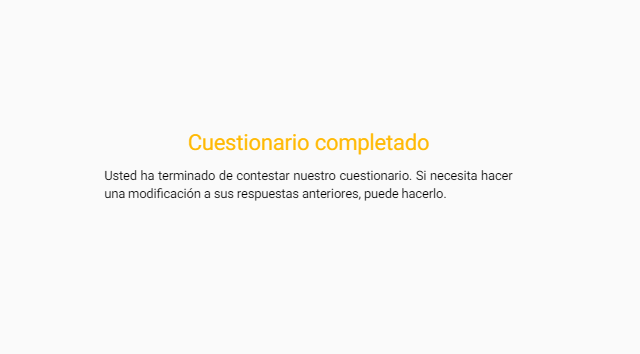
\includegraphics[scale=0.6]{images/Interfaz/MAT-34cuestionarioCompletado.png}
	\caption{Cuestionario completado}
	\end{figure}
\end{enumerate}

  \subsection{ER-01: Cancelar envío de las respuestas de la encuesta}
\begin{enumerate}
	\item Presione el botón \textbf{Continuar en el cuestionario}
  \begin{figure}[hbtp]
	
\includegraphics[scale=0.3]{images/Interfaz/MAT-34continuar.png}
	\caption{Continuar en el cuestionario}
	\end{figure}
\end{enumerate}

  